%  ################# Modelo de Relatório Analógica ##############################################
%   Author: Luiz Alberto Marinho
%   Descrição: Feito com base no modelo passado pelo professor Renê e com os pacotes ja prontos da 
%  norma ABNT desenvolvidos por: "abnTeX2 group". 
%       Dúvidas de como usar os pacotes da ABNT acessar: 
%   https://pt.overleaf.com/latex/templates/modelo-canonico-de-artigo-cientifico-com-abntex2/bycmpjrpdxnr
%       Acessar o arquivo chamado preambulo para ver os pacotes adicionados nesse documento
%
%
%
%
%

\documentclass[
	% -- opções da classe memoir --
	article,			% indica que é um artigo acadêmico
	11pt,				% tamanho da fonte
	oneside,			% para impressão apenas no verso. Oposto a twoside
	a4paper,			% tamanho do papel. 
	% -- opções da classe abntex2 --
	%chapter=TITLE,		% títulos de capítulos convertidos em letras maiúsculas
	%section=TITLE,		% títulos de seções convertidos em letras maiúsculas
	%subsection=TITLE,	% títulos de subseções convertidos em letras maiúsculas
	%subsubsection=TITLE % títulos de subsubseções convertidos em letras maiúsculas
	% -- opções do pacote babel --
	english,			% idioma adicional para hifenização
	brazil,				% o último idioma é o principal do documento
	sumario=tradicional
	]{abntex2}\usepackage{preambulo}

    % Títulos com fonte serifada (Latin Modern Roman)
\renewcommand{\ABNTEXchapterfont}{\rmfamily\bfseries}
\renewcommand{\ABNTEXsectionfont}{\rmfamily\bfseries}
\renewcommand{\ABNTEXsubsectionfont}{\rmfamily\bfseries}
\renewcommand{\ABNTEXsubsubsectionfont}{\rmfamily\bfseries}
\renewcommand{\ABNTEXsubsubsubsectionfont}{\rmfamily}
\usepackage{eso-pic}
\usepackage{transparent}
\usepackage{fancyhdr}
\usepackage{xcolor}


\begin{document}


\pagestyle{fancy}
\fancyhf{}
\fancyfoot[R]{\thepage}
\renewcommand{\headrulewidth}{0pt}
\renewcommand{\footrulewidth}{0pt}
\fancypagestyle{plain}{\fancyhf{}\fancyfoot[R]{\thepage}\renewcommand{\headrulewidth}{0pt}}

  
   % ----
    % Início do documento
    % ----
    
    \thispagestyle{empty}

\begin{center}
    
\includegraphics[scale=0.25]{Imagens/1.CAPA/brasao2_vertical_cor_300dpi.png}
    
    \vspace{2cm}
    
    \large\textbf{Disciplina de Proteção de Sistemas Elétricos de Potência}\\
    \small{Departamento de Engenharia Elétrica - UFC} \\
    \vfill
    \large \textbf{PROJETO FINAL}\\
    \vfill
    
    \flushleft{ 
        \textbf{Alunos:}\\  
        \hspace{0.5cm} Erika Oliveira Quinto - 511769\\
        \hspace{0.5cm} Luiz Alberto Silva Sales Marinho - 570920\\
        \hspace{0.5cm} Marcos Venicius de Oliveira Pinto - 500013\\
        \textbf{Professor:}\\
        \hspace{0.5cm} Raimundo Furtado Sampaio
    }
    
    \vspace*{0.5cm}
    
    \begin{center}
        2026.2
    \end{center}
\end{center}

\newpage % Muito importante para ir para a próxima página!
    
    \newpage
    \tableofcontents
    \newpage
    \newpage
\section{\textbf{Apresentação}}

% ===================== APRESENTAÇÃO =====================

O sistema de proteção de uma rede elétrica tem como função principal detectar condições anormais de operação, em especial os curtos-circuitos, e isolar o mais rapidamente possível apenas a parcela do sistema afetada pelo defeito, preservando a integridade dos equipamentos, a segurança das pessoas e a continuidade do fornecimento às demais cargas \cite{mamede2013}. Para que esse objetivo seja atingido, os dispositivos de proteção devem ser dimensionados e ajustados de forma a atender, simultaneamente, aos requisitos de seletividade, sensibilidade, rapidez e confiabilidade, além de operarem de maneira coordenada entre si \cite{kindermann2005}.

No Campus do Pici da Universidade Federal do Ceará (UFC) são desenvolvidas, além das atividades acadêmicas e administrativas, aulas práticas em laboratórios e diversos projetos de pesquisa e desenvolvimento, muitos dos quais dependem de um suprimento contínuo de energia elétrica \cite{silveira2022}. Nesse contexto, um estudo de proteção bem elaborado é fundamental para garantir que, na ocorrência de uma falta, seja desligado o menor número possível de cargas do campus, e por um tempo mínimo.

Até agosto de 2019, o Campus do Pici era atendido em média tensão (13,8~kV) pelo alimentador PCI01C8 da concessionária local, um alimentador praticamente exclusivo, que atendia apenas duas unidades consumidoras: o próprio Campus do Pici e o Núcleo de Tecnologia Industrial do Ceará (NUTEC) \cite{silveira2019apres}. 


Atualmente, o campus é suprido por uma subestação própria de 69-13,8~kV, denominada SE Campus do Pici, conectada ao Sistema de Distribuição em Alta Tensão (SDAT) da Enel Distribuição Ceará por meio de uma derivação da Linha de Distribuição de Alta Tensão (LDAT) 02L9, que interliga as subestações Pici (SED PCI, barra 7955) e Maguary (SED MGY, barra 9015). A Figura~\ref{fig:unifilar_simplificado} apresenta o diagrama unifilar simplificado do sistema, com os níveis de curto-circuito e as correntes máximas de carga e dos condutores dos alimentadores \cite{sampaio2026roteiro}.

\begin{figure}[htbp]
    \centering
    \caption{Diagrama unifilar simplificado da derivação da LDAT 02L9, da SE Campus do Pici e do Sistema de Distribuição em Média Tensão (SDMT) do campus.}
    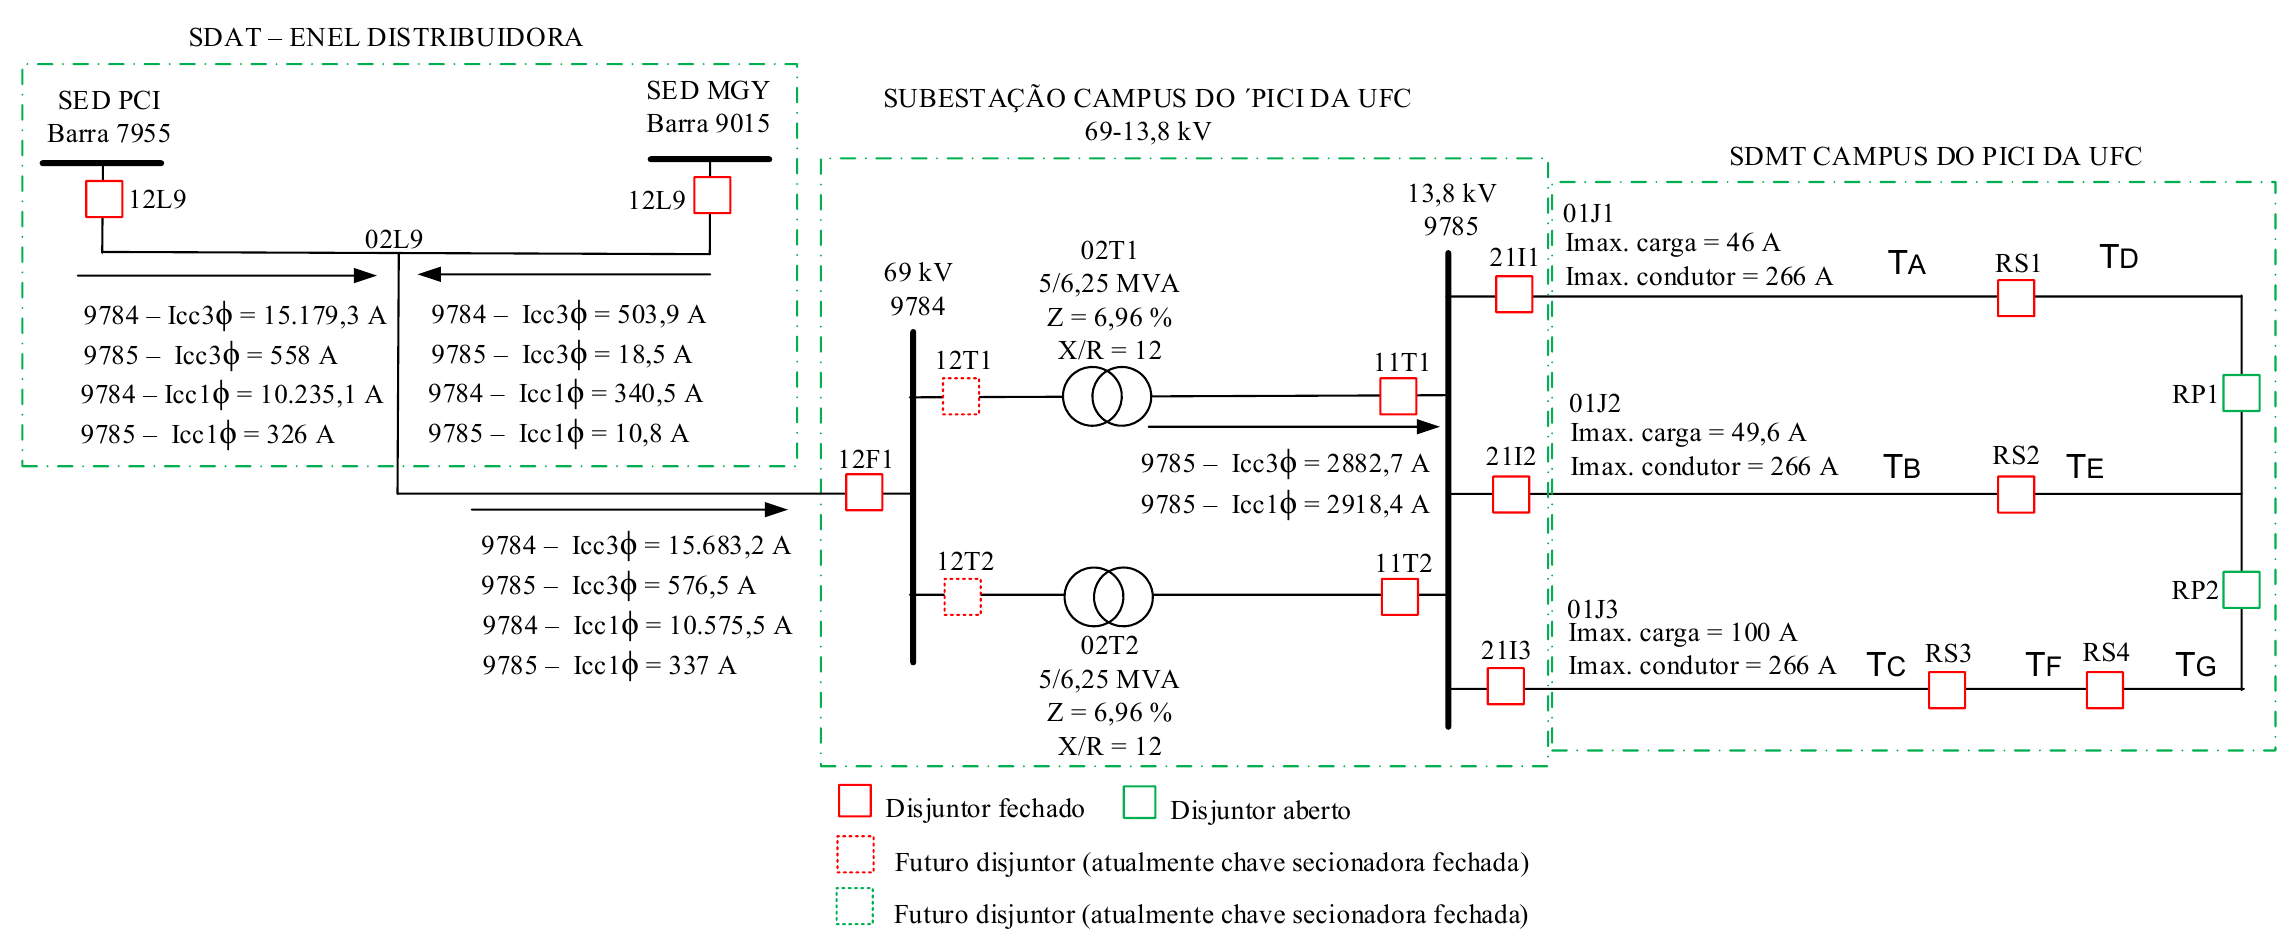
\includegraphics[width=16cm]{Imagens/unifilar_simplificado.png}
    \label{fig:unifilar_simplificado}
    \par\vspace{2pt}
    {\small Fonte: \cite{sampaio2026roteiro}.}
\end{figure}

A subestação é composta por um vão de entrada de linha em 69~kV, protegido pelo disjuntor 12F1, um barramento de 69~kV (barra 9784) e dois transformadores de potência, 02T1 e 02T2, de 5,00/6,25~MVA (ONAN/ONAF), com impedância de 6,96\%, relação $X/R = 12$ e ligação triângulo no primário e estrela aterrada no secundário (Dyn1). Do lado de alta tensão, os transformadores estão atualmente conectados ao barramento por chaves seccionadoras, estando prevista a instalação futura dos disjuntores 12T1 e 12T2. Do lado de média tensão, cada transformador se conecta ao barramento de 13,8~kV (barra 9785) por meio dos disjuntores gerais 11T1 e 11T2. As correntes nominais de cada transformador são de 41,8~A em 69~kV e 209,2~A em 13,8~kV na potência ONAN, e de 52,3~A e 261,5~A, respectivamente, na potência ONAF.

A distribuição em média tensão é feita por três alimentadores radiais, cujas saídas são protegidas pelos disjuntores 21I1, 21I2 e 21I3. Ao longo da rede estão instalados os religadores RS1, RS2, RS3 e RS4, normalmente fechados, que dividem os alimentadores nos trechos $T_A$ a $T_G$. Os pontos de interligação entre alimentadores, RP1 e RP2, operam normalmente abertos, o que confere à rede uma topologia radial com recurso, permitindo a transferência de carga entre alimentadores em situações de contingência. As correntes máximas de carga registradas nos alimentadores 01J1, 01J2 e 01J3 são de 46~A, 49,6~A e 100~A, respectivamente, e os condutores dos troncos possuem capacidade de condução de 266~A \cite{sampaio2026roteiro}.

Os níveis de curto-circuito nas barras da subestação, fornecidos pela concessionária, estão resumidos na Tabela~\ref{tab:niveis_cc}. Nota-se que a contribuição da SED PCI é largamente predominante sobre a da SED MGY. Destaca-se ainda que, por causa da ligação em triângulo do primário dos transformadores, a corrente de falta fase-terra na barra de 13,8~kV é vista no lado de 69~kV com apenas $1/\sqrt{3}$ do seu valor refletido pela relação de transformação, característica que influencia diretamente os ajustes das funções de neutro.

\begin{table}[htbp]
    \centering
    \caption{Níveis de curto-circuito nas barras da SE Campus do Pici, considerando os dois transformadores energizados.}
    \label{tab:niveis_cc}
    \begin{tabular}{lccc}
        \hline
        \textbf{Local da falta} & \textbf{Corrente medida em} & \textbf{$I_{cc3\phi}$ (A)} & \textbf{$I_{cc1\phi}$ (A)} \\
        \hline
        Barra 9784 (69 kV)   & 69 kV (entrada 12F1)   & 15.683,2 & 10.575,5 \\
        Barra 9785 (13,8 kV) & 69 kV (entrada 12F1)   & 576,5    & 337,0    \\
        Barra 9785 (13,8 kV) & 13,8 kV (barramento)   & 2.882,7  & 2.918,4  \\
        \hline
    \end{tabular}
    \par\vspace{2pt}
    {\small Fonte: adaptado de \cite{sampaio2026roteiro}.}
\end{table}

A montante da SE Campus do Pici, a proteção da saída de linha 12L9 da SED PCI é realizada por um relé SEL-411L, cujos ajustes constam na Ordem de Ajuste de Proteção (OAP) nº 046/2018 da concessionária. A função de sobrecorrente temporizada de fase (51) desse relé está ajustada com corrente de \textit{pick-up} de 1.161,6~A (RTC 1200-5), curva IEC muito inversa e dial de tempo 0,12, e a função de neutro (51N) com \textit{pick-up} de 160,8~A, mesma família de curva e dial 0,55 \cite{enel2018oap}. Para um curto-circuito trifásico na barra de 69~kV da subestação do campus, a função 51 da SED PCI opera em cerca de 0,13~s, o que impõe a principal restrição deste estudo: todas as proteções da SE Campus do Pici devem ser ajustadas abaixo das curvas da concessionária, respeitando os intervalos de coordenação estabelecidos.

Nos estudos realizados em 2018, a subestação teve sua proteção implementada com relés SEL-751 na entrada de linha (12F1), nos disjuntores gerais de barra (11T1 e 11T2) e nas saídas de alimentadores (21I1, 21I2 e 21I3), e com um relé SEL-787 na proteção diferencial dos transformadores \cite{ufc2018diagtempo}. A rede elétrica do campus já foi objeto de outros estudos de proteção, entre os quais se destacam o estudo das proteções do sistema elétrico do Campus do Pici realizado na própria disciplina \cite{andrade2016} e o trabalho de conclusão de curso que avaliou o impacto da integração de uma usina fotovoltaica sobre os ajustes da rede, considerando a operação de apenas um transformador \cite{silveira2022}. Diferentemente deste último, o presente projeto considera os dois transformadores energizados simultaneamente, condição que eleva os níveis de curto-circuito no barramento de 13,8~kV.

Diante do exposto, este projeto tem como objetivo realizar o estudo de coordenação e seletividade das proteções da SE Campus do Pici e das saídas dos alimentadores de distribuição em 13,8~kV, seguindo os critérios estabelecidos em \cite{sampaio2026roteiro}. Para isso, o trabalho está organizado da seguinte forma:

\begin{itemize}
    \item[--] apresentação do diagrama unifilar de proteção da subestação, com a identificação das funções de proteção associadas a cada disjuntor;
    \item[--] dimensionamento e especificação dos transformadores de corrente (TCs) pelos métodos da corrente nominal, do curto-circuito, da tensão máxima no secundário e de Stanley E. Zocholl;
    \item[--] estudo de coordenação das proteções de sobrecorrente (funções 50/51, 50/51N, 51NS, 46, 50BF e 79), englobando o cálculo dos ajustes, os coordenogramas, os diagramas de tempo e a elaboração das ordens de ajuste das proteções (OAP);
    \item[--] estudo da proteção diferencial dos transformadores (função 87T), contemplando as ligações e o dimensionamento dos TCs, o cálculo dos ajustes e a curva característica da função diferencial;
    \item[--] conclusões e proposição de melhorias para o sistema de proteção do campus.
\end{itemize}

Os ajustes foram desenvolvidos considerando as margens de coordenação de 0,4~s entre funções temporizadas (51-51 e 51N-51N), 0,2~s para a seletividade lógica, 0,25~s para a falha de disjuntor e 0,1~s para o tempo de operação das funções instantâneas \cite{sampaio2026roteiro}, bem como as características dos relés comerciais adotados \cite{sel2013sel751, abb1997tpu2000r} e os requisitos de IEDs de proteção estabelecidos pela concessionária \cite{enel2022et2178}.
    \newpage
\section{\textbf{Diagrama Unifilar de Proteção}}

Na Figura~\ref{fig:diagrama_unifilar_protecao} foi apresentada a configuração proposta para a proteção da SE Campus do Pici. Foram representados os equipamentos de manobra, os transformadores de corrente (TCs) e as funções de proteção identificadas por sua nomenclatura ANSI/IEEE C37.2. As cores distinguiram o setor de 69~kV (vermelho), o setor de 13,8~kV (azul) e a proteção dos transformadores de potência (magenta). O diagrama reuniu funções disponíveis nos vãos; sua representação não significou que todas tivessem sido habilitadas no mesmo grupo de ajustes.

\begin{figure}[htbp]
    \centering
    \caption{Diagrama unifilar de proteção da SE Campus do Pici.}
    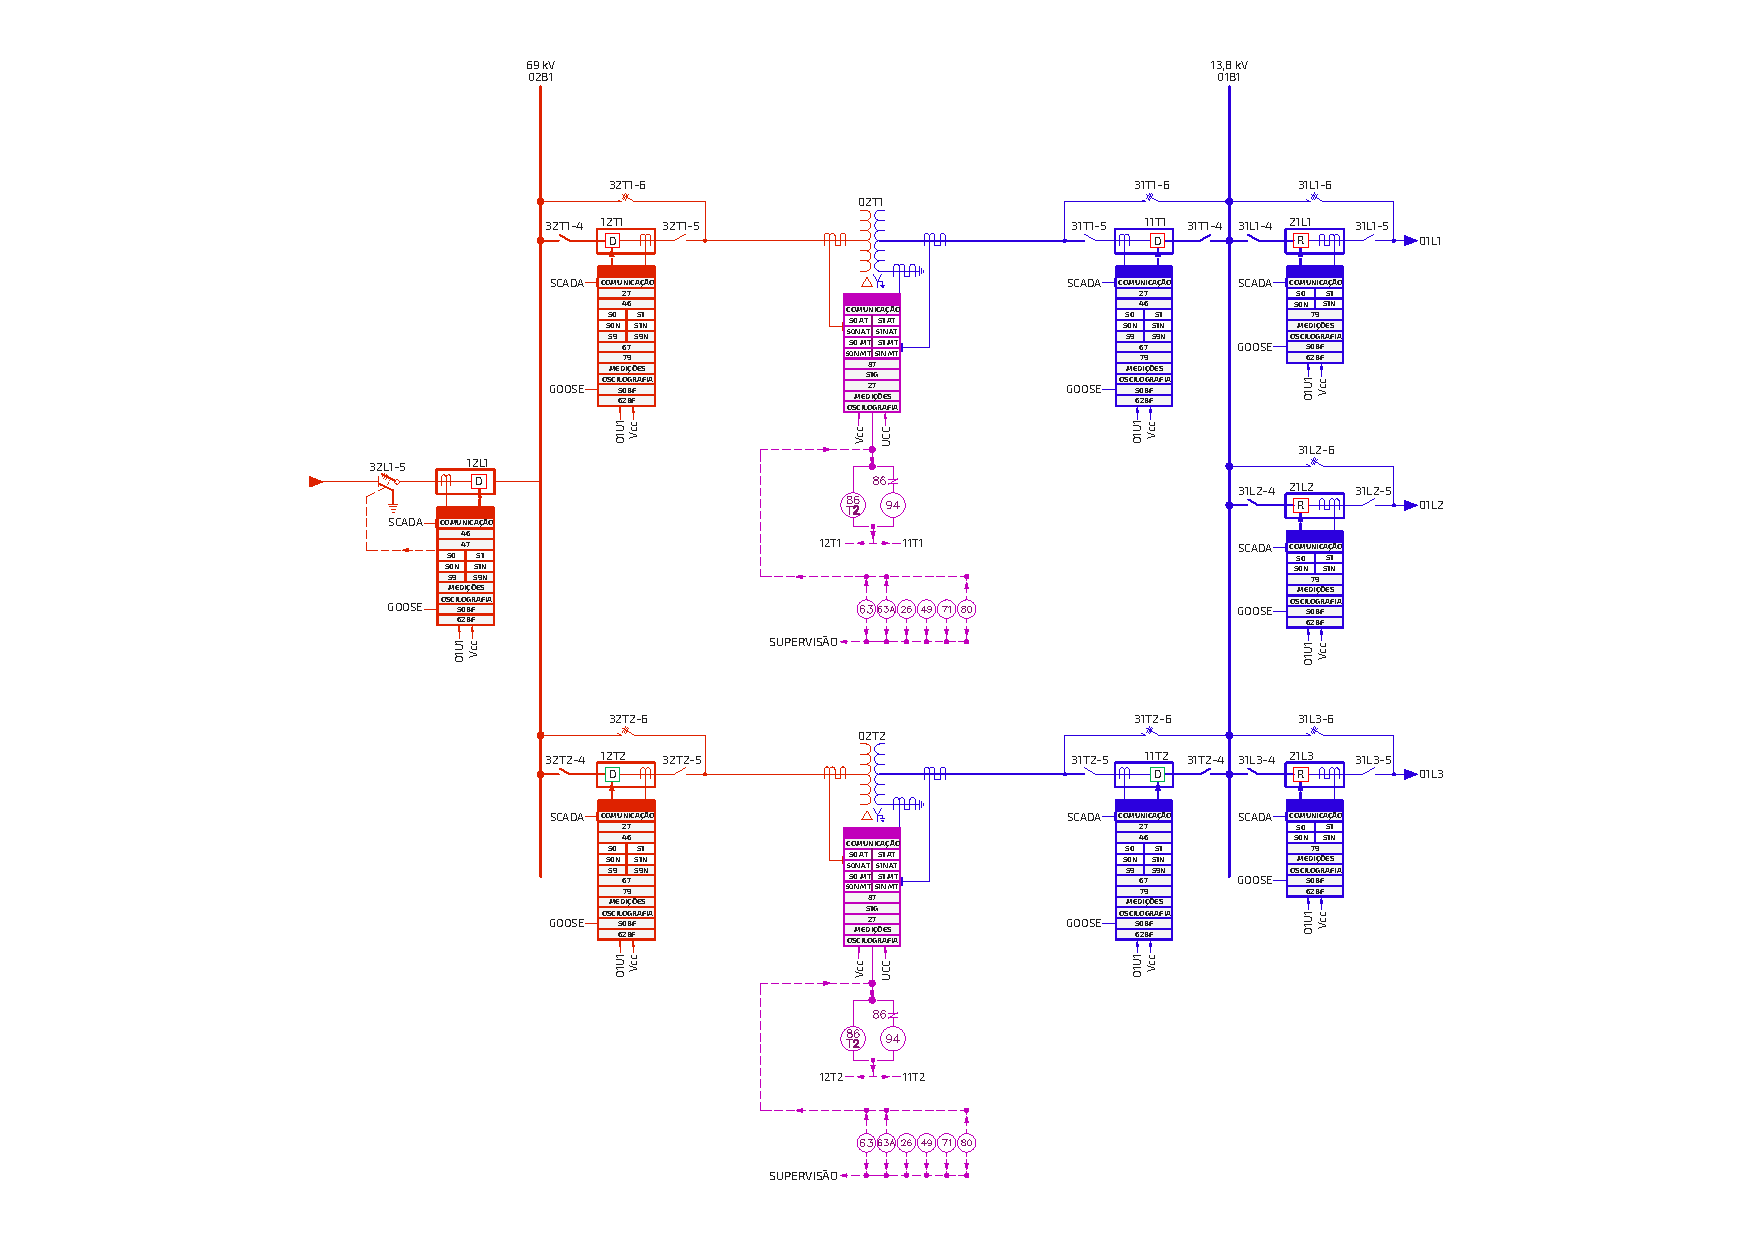
\includegraphics[width=16cm]{Imagens/Diagrama SEP.pdf}
    \label{fig:diagrama_unifilar_protecao}
    {\small Fonte: Elaborado pelos autores.}
\end{figure}

No setor de 69~kV, a entrada de linha foi associada ao disjuntor 12L1 e à chave seccionadora 32L1-5, com lâmina de aterramento. Foram representadas as funções de sobrecorrente de fase e de neutro (50/51 e 50N/51N), desequilíbrio de corrente (46), sequência de fase de tensão (47), sobretensão (59/59N) e falha de disjuntor (50BF/62BF). O barramento 02B1 foi associado aos transformadores 02T1 e 02T2 por meio dos disjuntores 12T1 e 12T2, incorporados à proposta, e de suas seccionadoras de isolamento e de \textit{by-pass}. Foram mantidas apenas as funções habilitadas nas OAPs calculadas. Em particular, os estágios 50/50N da entrada foram desabilitados no grupo estudado, e o religamento automático dos vãos dos transformadores não foi habilitado.

Para cada transformador foi prevista proteção diferencial (87T) com medição nos dois lados, conforme a especificação da seção correspondente. A proteção de sobrecorrente de retaguarda foi associada aos IEDs dos respectivos vãos, e a função 51G foi associada ao TC dedicado do neutro do enrolamento em estrela aterrada. Foi prevista a abertura dos disjuntores dos dois lados da unidade protegida, 12T1/11T1 ou 12T2/11T2, para atuação diferencial ou das proteções intrínsecas com comando de desligamento. O bloqueio 86T foi utilizado para impedir reenergização após atuação das proteções selecionadas. A função 94 foi identificada como função auxiliar de disparo, distinta do circuito de antibombeamento. Os dispositivos intrínsecos representados no diagrama não foram objeto de cálculo de ajustes elétricos neste estudo.

No setor de 13,8~kV, os transformadores foram associados ao barramento 01B1 pelos disjuntores gerais 11T1 e 11T2. Foram utilizadas as funções temporizadas de fase e de neutro nos gerais, e foram desabilitados seus estágios 50/50N no grupo estudado. Desse barramento foram representadas as saídas 01L1, 01L2 e 01L3, protegidas pelos equipamentos 21L1, 21L2 e 21L3. Nos alimentadores foram considerados sobrecorrente de fase e de neutro, neutro sensível, desequilíbrio, religamento e falha de disjuntor, conforme os ajustes da seção seguinte. As chaves de \textit{by-pass} foram mantidas no diagrama, mas sua utilização não foi incluída na topologia normal de cálculo.

Foi prevista alimentação dos IEDs em corrente contínua pelo sistema de serviços auxiliares O1U1 e integração ao SCADA. Para a troca de sinais de proteção foram consideradas mensagens GOOSE entre equipamentos com interface IEC 61850 compatível, ou contatos e interfaces apropriadas nos demais casos, sem pressupor suporte nativo ao mesmo protocolo em todos os modelos. A definição dos circuitos de disparo, dos caminhos de comunicação e de seus atrasos foi vinculada ao comissionamento. Foram preservados os recursos de medição e oscilografia para análise das perturbações. O único transformador em serviço e os pontos RP1/RP2 normalmente abertos definiram a topologia radial utilizada nos cálculos.

    \newpage
\section{\textbf{Dimensionamento e especificação dos TCs}}

% ===================== DIMENSIONAMENTO E ESPECIFICAÇÃO DOS TCs =====================

Os transformadores de corrente (TCs) reproduzem, em seu secundário, uma imagem reduzida das correntes primárias, para que os relés de proteção possam medi-las. Para que a proteção opere corretamente, o TC deve suportar a corrente de carga em regime permanente e reproduzir as correntes de curto-circuito sem saturar, de modo que o relé receba um sinal fiel à corrente de falta \cite{mamede2013}.

Nesta seção são dimensionados os TCs de proteção de sobrecorrente da SE Campus do Pici, identificados no diagrama unifilar da Figura~\ref{fig:diagrama_unifilar_protecao}: os TCs de fase do vão de entrada de linha (12L1), dos disjuntores de alta tensão dos transformadores (12T1 e 12T2), dos disjuntores gerais de média tensão (11T1 e 11T2) e das saídas dos alimentadores (21L1, 21L2 e 21L3), além do TC de neutro dos transformadores, utilizado pela função 51G. Os TCs associados à proteção diferencial dos transformadores são tratados na seção referente à função 87T.

No dimensionamento, considerou-se a operação da subestação com apenas um transformador energizado, permanecendo o outro como reserva. Os TCs dos dois transformadores recebem a mesma especificação, de modo que qualquer um deles possa entrar em operação sem alteração nos ajustes da proteção.

\subsection{Dados de projeto}

Os TCs disponíveis para os setores de alta e média tensão da subestação são apresentados na Tabela~\ref{tab:tc_disponiveis}. Todos são do tipo multirrelação, com fator de sobrecorrente $FS = 20$, fator térmico $FT = 1{,}2$ e classe de exatidão 10B200, isto é, erro máximo de 10\% para uma tensão secundária de até 200~V, desenvolvida com 20 vezes a corrente nominal secundária (100~A) circulando na carga nominal de 2~$\Omega$.

\begin{table}[htbp]
    \centering
    \caption{Transformadores de corrente disponíveis para a SE Campus do Pici.}
    \label{tab:tc_disponiveis}
    \begin{tabular}{ccccc}
        \hline
        \textbf{Nível de tensão} & \textbf{Relação nominal (A)} & \textbf{FS} & \textbf{FT} & \textbf{Exatidão} \\
        \hline
        69 kV   & 200/400/600-5          & 20 & 1,2 & 10B200 \\
        \hline
        \multirow{3}{*}{13,8 kV} & 800/1000/1200/1400-5 & 20 & 1,2 & 10B200 \\
                                 & 200/400-5            & 20 & 1,2 & 10B200 \\
                                 & 100/200/400/600/800-5 & 20 & 1,2 & 10B200 \\
        \hline
    \end{tabular}
    \par\vspace{2pt}
    {\small Fonte: \cite{sampaio2026roteiro}.}
\end{table}

A carga conectada ao secundário de cada TC é formada pelos condutores que o interligam ao relé na casa de comando e pela carga do próprio relé. Os dados utilizados estão na Tabela~\ref{tab:dados_carga_tc}.

\begin{table}[htbp]
    \centering
    \caption{Dados dos condutores secundários e do relé.}
    \label{tab:dados_carga_tc}
    \begin{tabular}{lcc}
        \hline
        \textbf{Dado} & \textbf{Pátio de 69 kV} & \textbf{Pátio de 13,8 kV} \\
        \hline
        Comprimento dos condutores ($L$)  & 100 m & 80 m \\
        Impedância dos condutores ($Z_c$) & $(5{,}52 + j0{,}13)~\Omega$/km & $(5{,}52 + j0{,}13)~\Omega$/km \\
        Carga do relé ($S_r$)             & 0,2 VA & 0,2 VA \\
        \hline
    \end{tabular}
    \par\vspace{2pt}
    {\small Fonte: \cite{sampaio2026roteiro}.}
\end{table}

A impedância do relé, referida à corrente nominal secundária de 5~A, é dada por:

\begin{equation}
    Z_r = \frac{S_r}{I_{sec}^2} = \frac{0{,}2}{5^2} = 0{,}008~\Omega
\end{equation}

A impedância total no secundário do TC é calculada pela Equação~\eqref{eq:z_total}. Considera-se o percurso de ida e volta dos condutores ($2L$), que corresponde à condição mais severa, verificada nas faltas fase-terra, quando a corrente retorna pelo condutor de neutro do circuito secundário. A resistência interna do enrolamento secundário do TC foi desprezada, por não ter sido fornecida.

\begin{equation}
    Z_{TC} = 2 \cdot L \cdot Z_c + Z_r
    \label{eq:z_total}
\end{equation}

\begin{itemize}
    \item[--] Pátio de 69 kV: $Z_{TC} = 2 \cdot 0{,}100 \cdot (5{,}52 + j0{,}13) + 0{,}008 = 1{,}112 + j0{,}026~\Omega \Rightarrow |Z_{TC}| = 1{,}1123~\Omega$;
    \item[--] Pátio de 13,8 kV: $Z_{TC} = 2 \cdot 0{,}080 \cdot (5{,}52 + j0{,}13) + 0{,}008 = 0{,}8912 + j0{,}0208~\Omega \Rightarrow |Z_{TC}| = 0{,}8914~\Omega$.
\end{itemize}

As correntes máximas de carga e de curto-circuito consideradas para cada TC estão resumidas na Tabela~\ref{tab:correntes_tc}, adotando-se os seguintes critérios:

\begin{itemize}
    \item[--] \textbf{12L1}: com apenas um transformador energizado, a corrente de carga corresponde à corrente nominal ONAF desse transformador em 69~kV (52,3~A), e a corrente de curto-circuito máxima é a falta trifásica no barramento de 69~kV (15.683,2~A);
    \item[--] \textbf{12T1 e 12T2}: a corrente de carga é a corrente nominal ONAF de cada transformador em 69~kV (52,3~A). A corrente de curto-circuito máxima ocorre para uma falta nos terminais de alta tensão do transformador, alimentada pelo barramento de 69~kV, e é igual à corrente de falta trifásica nessa barra (15.683,2~A);
    \item[--] \textbf{11T1 e 11T2}: a corrente de carga é a corrente nominal ONAF do transformador em 13,8~kV (261,5~A). Como apenas um transformador está em operação, toda a corrente de falta no barramento de 13,8~kV circula pelo seu disjuntor geral, e a corrente de curto-circuito máxima é a falta fase-terra nessa barra (2.918,4~A);
    \item[--] \textbf{21L1, 21L2 e 21L3}: como os relés dos alimentadores devem ter o mesmo ajuste \cite{sampaio2026roteiro}, adotou-se a maior corrente de carga registrada entre os alimentadores (100~A). A corrente de curto-circuito máxima é a falta fase-terra no barramento de 13,8~kV (2.918,4~A);
    \item[--] \textbf{Neutro dos transformadores}: em regime normal, o TC de neutro conduz apenas a corrente de desequilíbrio. Sua corrente máxima é a corrente residual ($3I_0$) da falta fase-terra no barramento de 13,8~kV, que retorna integralmente pelo neutro do transformador em operação (2.918,4~A).
\end{itemize}

\begin{table}[htbp]
    \centering
    \caption{Correntes máximas de carga e de curto-circuito consideradas no dimensionamento dos TCs.}
    \label{tab:correntes_tc}
    \begin{tabular}{lccc}
        \hline
        \textbf{TC} & \textbf{Tensão (kV)} & \textbf{$I_{carga,máx}$ (A)} & \textbf{$I_{cc,máx}$ (A)} \\
        \hline
        12L1                 & 69   & 52,3  & 15.683,2 \\
        12T1 e 12T2          & 69   & 52,3  & 15.683,2 \\
        11T1 e 11T2          & 13,8 & 261,5 & 2.918,4 \\
        21L1, 21L2 e 21L3    & 13,8 & 100,0 & 2.918,4 \\
        Neutro 02T1 e 02T2   & 13,8 & --    & 2.918,4 \\
        \hline
    \end{tabular}
    \par\vspace{2pt}
    {\small Fonte: elaborado pelos autores.}
\end{table}

\subsection{Critérios de dimensionamento}

Os TCs foram dimensionados segundo os quatro critérios estabelecidos em \cite{sampaio2026roteiro}, descritos a seguir.

\textbf{a) Critério da corrente nominal}: a corrente primária nominal do TC ($I_p$) deve ser maior ou igual à corrente máxima de carga. Verifica-se também se a corrente admissível em regime permanente, dada pelo fator térmico, atende à carga máxima:

\begin{equation}
    I_p \geq I_{carga,máx} \qquad \text{e} \qquad FT \cdot I_p \geq I_{carga,máx}
    \label{eq:crit_nominal}
\end{equation}

\textbf{b) Critério do curto-circuito}: a corrente primária nominal do TC multiplicada pelo fator de sobrecorrente deve ser maior ou igual à corrente máxima de curto-circuito:

\begin{equation}
    FS \cdot I_p \geq I_{cc,máx} \quad \Rightarrow \quad I_p \geq \frac{I_{cc,máx}}{20}
    \label{eq:crit_cc}
\end{equation}

\textbf{c) Critério da tensão máxima no secundário}: a tensão desenvolvida no secundário do TC durante o curto-circuito máximo deve ser menor que a tensão nominal da classe de exatidão ($V_N = 200$~V):

\begin{equation}
    V_s = \frac{I_{cc,máx}}{RTC} \cdot |Z_{TC}| \leq V_N
    \label{eq:crit_tensao}
\end{equation}

\textbf{d) Critério de Stanley E. Zocholl}: verifica se o TC reproduz, sem saturar, a corrente de curto-circuito com a máxima componente contínua (assimetria total). O critério é expresso por:

\begin{equation}
    20 \geq \left(\frac{X}{R} + 1\right) \cdot I_f \cdot Z_b
    \label{eq:zocholl}
\end{equation}

\noindent em que $I_f$ é a corrente máxima de falta no secundário do TC em pu da corrente nominal secundária e $Z_b$ é a carga do TC em pu da carga nominal da classe de exatidão. Detalhando os termos:

\begin{equation}
    20 \geq \left(\frac{X}{R} + 1\right) \cdot \left(\frac{I_{cc,máx,sec}}{I_{TC,sec}}\right) \cdot \left(\frac{Z_{TC}}{\dfrac{V_{TC,máx}}{20 \cdot I_{TC,sec}}}\right)
    \label{eq:zocholl_detalhada}
\end{equation}

Para a classe 10B200, a carga nominal é $V_{TC,máx}/(20 \cdot I_{TC,sec}) = 200/(20 \cdot 5) = 2~\Omega$. Foi adotada a relação $X/R = 12{,}77$ \cite{sampaio2026roteiro}.

Entre as relações que atendem aos critérios a, b e c, foi escolhida a menor. Uma RTC menor resulta em correntes secundárias maiores para um mesmo valor primário, o que permite ajustar as funções de neutro (51N, 51NS e 51G) com valores de \textit{pick-up} reduzidos, dentro das faixas de ajuste do relé \cite{sel2013sel751}.

\subsection{Dimensionamento do TC do disjuntor de entrada 12L1}

\textbf{a) Critério da corrente nominal}

\begin{equation*}
    I_p \geq 52{,}3~\text{A}
\end{equation*}

Pelo critério da corrente nominal, a menor relação disponível (200-5) já seria suficiente.

\textbf{b) Critério do curto-circuito}

\begin{equation*}
    I_p \geq \frac{15.683{,}2}{20} = 784{,}2~\text{A}
\end{equation*}

A maior relação disponível para 69~kV é 600-5. Como $20 \cdot 600 = 12.000~\text{A} < 15.683{,}2~\text{A}$, o critério do curto-circuito não é atendido por nenhum dos TCs disponíveis para esse nível de tensão. Assim, adotou-se a maior relação, 600-5 ($RTC = 120$), e sua adequação foi verificada pelo critério da tensão máxima no secundário.

\textbf{c) Critério da tensão máxima no secundário}

\begin{equation*}
    V_s = \frac{15.683{,}2}{120} \cdot 1{,}1123 = 130{,}69 \cdot 1{,}1123 = 145{,}4~\text{V} \leq 200~\text{V}
\end{equation*}

O critério é atendido. Embora a corrente de falta corresponda a 26,1 vezes a corrente nominal do TC, a carga real conectada ao secundário (1,11~$\Omega$) é praticamente a metade da carga nominal da classe (2~$\Omega$). Por isso, o TC pode conduzir até $200/(5 \cdot 1{,}1123) = 35{,}96$ vezes sua corrente nominal sem ultrapassar a tensão de 200~V, ou seja, ele reproduz a corrente de falta simétrica sem saturar.

\textbf{d) Critério de Stanley E. Zocholl}

\begin{equation*}
    I_f = \frac{130{,}69}{5} = 26{,}14~\text{pu} \qquad Z_b = \frac{1{,}1123}{2} = 0{,}5562~\text{pu}
\end{equation*}

\begin{equation*}
    \left(12{,}77 + 1\right) \cdot 26{,}14 \cdot 0{,}5562 = 200{,}2 > 20
\end{equation*}

O critério de Zocholl não é atendido, o que indica que o TC pode saturar durante os primeiros ciclos de um curto-circuito com assimetria máxima.

\subsection{Dimensionamento dos demais TCs}

Os demais TCs foram dimensionados com o mesmo procedimento, e os resultados estão resumidos na Tabela~\ref{tab:resultados_tc}.

\begin{table}[htbp]
    \centering
    \caption{Resultados dos critérios de dimensionamento dos TCs.}
    \label{tab:resultados_tc}
    \resizebox{\textwidth}{!}{%
    \begin{tabular}{lccccccccc}
        \hline
        \multirow{2}{*}{\textbf{TC}} & \multirow{2}{*}{\textbf{RTC}} & \multicolumn{2}{c}{\textbf{a) Corrente nominal}} & \multicolumn{2}{c}{\textbf{b) Curto-circuito}} & \multicolumn{2}{c}{\textbf{c) Tensão no secundário}} & \multicolumn{2}{c}{\textbf{d) Zocholl}} \\
         & & $I_p \geq I_{carga}$ & Atende? & $I_{cc}/20$ (A) & Atende? & $V_s$ (V) & Atende? & Resultado & Atende? \\
        \hline
        12L1               & 600-5 (120) & $600 \geq 52{,}3$  & Sim & 784,2 & Não & 145,4 & Sim & 200,2 & Não \\
        12T1 e 12T2        & 600-5 (120) & $600 \geq 52{,}3$  & Sim & 784,2 & Não & 145,4 & Sim & 200,2 & Não \\
        11T1 e 11T2        & 400-5 (80)  & $400 \geq 261{,}5$ & Sim & 145,9 & Sim & 32,5  & Sim & 44,8  & Não \\
        21L1, 21L2 e 21L3  & 200-5 (40)  & $200 \geq 100{,}0$ & Sim & 145,9 & Sim & 65,0  & Sim & 89,6  & Não \\
        Neutro 02T1 e 02T2 & 200-5 (40)  & --                 & --  & 145,9 & Sim & 65,0  & Sim & 89,6  & Não \\
        \hline
    \end{tabular}}
    \par\vspace{2pt}
    {\small Fonte: elaborado pelos autores.}
\end{table}

Para os TCs 12T1 e 12T2, assim como para o TC 12L1, a corrente de carga de 52,3~A seria atendida pela relação 200-5. No entanto, como esses TCs estão sujeitos à mesma corrente de falta do TC 12L1, foi adotada a relação 600-5, que é a única que atende ao critério da tensão máxima no secundário. Com essa relação, uma corrente de \textit{pick-up} da função 51 de $1{,}25 \times 52{,}3 = 65{,}4$~A corresponde a 0,545~A no secundário, ainda acima do valor mínimo de ajuste do relé SEL-751 para TCs de 5~A (0,50~A) \cite{sel2013sel751}.

Para os TCs 11T1 e 11T2, a relação 400-5 é a menor que atende à corrente nominal ONAF do transformador. Essa relação também atende à soma das cargas máximas dos três alimentadores ($46 + 49{,}6 + 100 = 195{,}6$~A), suprida integralmente pelo transformador em operação. Seu limite térmico em regime permanente ($1{,}2 \times 400 = 480$~A) comporta ainda a sobrecarga admissível do transformador considerada no ajuste da função 51 (até $1{,}5 \times 261{,}5 = 392{,}2$~A).

Para os TCs dos alimentadores, a relação 200-5 atende à maior corrente de carga registrada (100~A) e ao critério do curto-circuito ($20 \times 200 = 4.000~\text{A} \geq 2.918{,}4~\text{A}$). Seu limite térmico em regime permanente ($1{,}2 \times 200 = 240$~A) é superior à soma das cargas máximas dos três alimentadores ($46 + 49{,}6 + 100 = 195{,}6$~A). Dessa forma, o TC suporta inclusive a transferência de toda a carga do campus para um único alimentador por meio dos pontos de interligação RP1 e RP2. Como os TCs são multirrelação, a derivação pode ser alterada para 400-5 caso a carga dos alimentadores cresça até valores próximos da capacidade dos condutores (266~A).

\subsection{Análise do critério de Zocholl}

Nenhum dos TCs atende ao critério de Zocholl. Isso indica que, para curtos-circuitos próximos à subestação com assimetria máxima, os TCs podem saturar nos primeiros ciclos da falta, enquanto a componente contínua da corrente não se extingue. Para a relação $X/R = 12{,}77$, a constante de tempo dessa componente é:

\begin{equation}
    \tau = \frac{X/R}{2 \pi f} = \frac{12{,}77}{2 \pi \cdot 60} = 33{,}9~\text{ms}
\end{equation}

\noindent ou seja, a componente contínua é praticamente extinta após cerca de $5\tau \approx 170$~ms. Assim, a saturação transitória tende a afetar pouco as funções temporizadas (51 e 51N), cujos tempos de operação para as correntes de falta em questão são da ordem de centenas de milissegundos, e afeta principalmente as funções instantâneas (50 e 50N), que podem ter a operação retardada nos primeiros ciclos da falta.

No setor de 13,8~kV, o critério seria atendido com a redução da carga secundária para valores de até 0,40~$\Omega$ (TCs 11T1 e 11T2) e 0,20~$\Omega$ (TCs dos alimentadores e de neutro), o que pode ser obtido com o aumento da seção dos condutores secundários ou a redução da distância entre os TCs e os relés. No setor de 69~kV, mesmo com a relação de 600-5, a carga secundária teria de ser inferior a 0,11~$\Omega$, valor menor que a impedância dos próprios condutores, o que exigiria TCs de classe de exatidão superior. Essas alternativas são discutidas na seção de proposição de melhorias.

\subsection{Especificação dos TCs}

A especificação final dos TCs de proteção de sobrecorrente da SE Campus do Pici é apresentada na Tabela~\ref{tab:especificacao_tc}.

\begin{table}[htbp]
    \centering
    \caption{Especificação dos TCs de proteção de sobrecorrente da SE Campus do Pici.}
    \label{tab:especificacao_tc}
    \resizebox{\textwidth}{!}{%
    \begin{tabular}{lccccccc}
        \hline
        \textbf{TC} & \textbf{Qtd.} & \textbf{Tensão (kV)} & \textbf{Relação nominal (A)} & \textbf{Derivação (RTC)} & \textbf{FS} & \textbf{FT} & \textbf{Exatidão} \\
        \hline
        12L1               & 3 & 69   & 200/400/600-5         & 600-5 (120) & 20 & 1,2 & 10B200 \\
        12T1 e 12T2        & 6 & 69   & 200/400/600-5         & 600-5 (120) & 20 & 1,2 & 10B200 \\
        11T1 e 11T2        & 6 & 13,8 & 200/400-5             & 400-5 (80)  & 20 & 1,2 & 10B200 \\
        21L1, 21L2 e 21L3  & 9 & 13,8 & 100/200/400/600/800-5 & 200-5 (40)  & 20 & 1,2 & 10B200 \\
        Neutro 02T1 e 02T2 & 2 & 13,8 & 100/200/400/600/800-5 & 200-5 (40)  & 20 & 1,2 & 10B200 \\
        \hline
    \end{tabular}}
    \par\vspace{2pt}
    {\small Fonte: elaborado pelos autores.}
\end{table}

    \newpage
\section{\textbf{Estudo de coordenação das proteções de sobrecorrente}}

\subsection{Cálculo dos ajuste das proteções de sobrecorrente}

\subsection{Coordenagrama}

\subsection{Diagrama de tempo}

\subsection{Ordem de ajuste das proteções (OAP)}
    \newpage
\section{\textbf{Estudo de seletividade da proteção diferencial do transformador}}

\subsection{Ligações, dimensionamento e especificação dos transformadores de corrente}

\subsection{Cálculo dos ajustes da função diferencial do transformador}

\subsection{Gerar a curva da função diferencial}
    \newpage
\section{\textbf{Conclusões}}

O estudo foi desenvolvido para a SE Campus do Pici com um transformador energizado e outro em reserva, mantendo-se os níveis de curto-circuito fornecidos pelo professor e incorporando-se os disjuntores de alta tensão dos transformadores à configuração proposta. Os critérios do roteiro foram relacionados aos parâmetros da apresentação sobre proteção de subestações de 69--13,8~kV, sem transferência dos dados de potência, cabos ou curto-circuito do exemplo para a instalação estudada.

Na revisão dos TCs de alta tensão, foram adotados 1200-5 na entrada 12L1 e 800-5 em 12T1, 12T2 e nos núcleos exclusivos de alta da proteção diferencial. Foram mantidos 400-5 nos gerais de média tensão e 200-5 nos alimentadores e nos neutros. As novas relações de alta atenderam aos três critérios calculados, com limites de curto de 24.000 e 16.000~A, superiores a 15.683,2~A. A insuficiência anterior do critério de curto foi resolvida, tendo permanecido necessária a confirmação das classes, da excitação e da suportabilidade dos equipamentos especificados.

Na sobrecorrente, foram adotadas curvas IEC muito inversas C2, com alvos iniciais de aproximadamente 0,20 e 0,30~s para fase e neutro dos alimentadores. Os ajustes secundários foram recalculados para os novos TCs, com arredondamento ao passo de 0,01~A e atualização dos valores primários efetivos. Os dials e aditivos permitiram manter margens nominais superiores ou iguais a 0,40~s entre as funções temporizadas locais nos intervalos verificados, inclusive no patamar de múltiplo máximo. Foram utilizados 24~A nos alimentadores, 60~A nos gerais e no neutro do transformador, 60,8~A no primário e 120~A na entrada.

A função 50 de fase do primário foi ajustada acima da corrente passante refletida acrescida do fator de assimetria de 1,73, com atraso de 0,05~s. Nos gerais de média tensão e na entrada, os estágios de alta corrente foram mantidos desabilitados, conforme a configuração de referência dos slides. Nos alimentadores, os valores calculados a partir de 80\% da corrente máxima foram classificados como pré-ajustes, sem comprovação de alcance ao longo da rede. A liberação desses estágios permaneceu dependente das correntes de falta até o primeiro religador.

Para a proteção diferencial, foram adotados os parâmetros de sensibilidade e dupla inclinação apresentados nos slides, com compensação do grupo Dyn1 e utilização de um IED compatível com o casamento das correntes e a sensibilidade requerida. A análise das faltas externas foi realizada com correntes compensadas, sem atribuição de corrente residual ao lado em triângulo. A característica percentual e os pontos de operação foram definidos analiticamente e representados na Figura~\ref{fig:87_caracteristica_diferencial}, sem atribuição de ensaios ou simulações transitórias não realizados.

A seletividade integral com a concessionária não foi demonstrada para as faltas do setor de 69~kV. A atuação de fase de Pici em aproximadamente 0,134~s e a proteção de distância existente impuseram restrições que não foram resolvidas apenas pelos ajustes locais. Os tempos típicos de processamento e interrupção dos slides reforçaram a necessidade de conferir o tempo total de eliminação, em lugar de comparar somente os atrasos intencionais.

Dessa forma, foi estabelecida uma proposta de ajustes e de coordenação local, com identificação das condições de aplicação e das limitações. A conclusão da verificação da rede completa permaneceu dependente dos curtos mínimos, dos ajustes dos religadores, do histórico de desequilíbrio, das características efetivas dos TCs e dos tempos dos disjuntores. As expressões e tabelas foram complementadas pelos coordenogramas, pelos diagramas de tempo e pela característica diferencial, mantendo-se as condições de aplicação dos ajustes representados.

    \newpage
\section{\textbf{Proposição de melhorias}}


    \newpage
% Referências bibliográficas
% ----------------------------------------------------------
\printbibliography

% ----------------------------------------------------------
% Anexos
% ----------------------------------------------------------
\begin{anexosenv}
    \clearpage
\renewcommand{\thesection}{\Alph{section}}
\refstepcounter{section}
\section*{\textbf{ANEXO~\thesection\ --- Código MATLAB para geração das ilustrações}}
\addcontentsline{toc}{section}{ANEXO~\thesection\ --- Código MATLAB para geração das ilustrações}
\label{anexo:codigo_matlab}

Foi preparado o arquivo \texttt{gerar\_ilustracoes.m}, apresentado na Listagem~\ref{lst:matlab_ilustracoes}, para reproduzir os coordenogramas, os diagramas de tempo, a temporização de falha de disjuntor e a característica diferencial dos capítulos 4 e 5. Os ajustes finais foram reunidos em matrizes, e as operações comuns de cálculo e representação foram agrupadas em funções locais. Foi incluída a conferência dos tempos nominais de referência, mantendo-se a distinção entre os pré-ajustes, as características temporizadas e a estimativa analítica de 51N de Pici.

Para contornar a falha de gravação observada na pasta utilizada para download, a exportação foi configurada para uma pasta temporária do sistema, com arquivos PNG a 300~dpi e PDF vetorial \cite{mathworks2026exportgraphics}. Foi prevista a leitura de cada PNG e a verificação dos marcadores inicial e final dos PDFs. Em seguida, foi prevista a compactação, a extração do ZIP e a comparação dos arquivos byte a byte, antes de sua cópia para a pasta de saída \cite{mathworks2026zip}. A conferência dos marcadores do PDF foi tratada como verificação básica de estrutura, complementada pela abertura e inspeção visual do arquivo.

Foi prevista a execução em MATLAB com suporte a \texttt{exportgraphics}, sem utilização de ferramentas adicionais de proteção. Com o arquivo na pasta atual ou no caminho de busca do MATLAB, a chamada foi definida por:

\begin{lstlisting}[language=Matlab,numbers=none]
arquivoZIP = gerar_ilustracoes;
\end{lstlisting}

No MATLAB Online, foi previsto o download do ZIP indicado ao término da execução, seguido de sua extração no computador. A pasta de saída também pôde ser informada como argumento da função.

\begingroup
\SingleSpacing
\renewcommand{\lstlistingname}{Listagem}
\lstinputlisting[
    language=Matlab,
    basicstyle=\ttfamily\footnotesize,
    keywordstyle=\bfseries\color{blue!60!black},
    commentstyle=\itshape\color{black!60},
    stringstyle=\color{black},
    numbers=left,
    numberstyle=\tiny\color{black!60},
    numbersep=6pt,
    columns=fullflexible,
    keepspaces=true,
    upquote=true,
    breaklines=true,
    showstringspaces=false,
    caption={Código MATLAB para geração das oito ilustrações e conferência da exportação.},
    label={lst:matlab_ilustracoes},
    literate=
        {á}{{\'a}}1 {à}{{\`a}}1 {â}{{\^a}}1 {ã}{{\~a}}1
        {é}{{\'e}}1 {ê}{{\^e}}1 {í}{{\'i}}1
        {ó}{{\'o}}1 {ô}{{\^o}}1 {õ}{{\~o}}1
        {ú}{{\'u}}1 {ç}{{\c c}}1
        {Á}{{\'A}}1 {À}{{\`A}}1 {Â}{{\^A}}1 {Ã}{{\~A}}1
        {É}{{\'E}}1 {Ê}{{\^E}}1 {Í}{{\'I}}1
        {Ó}{{\'O}}1 {Ô}{{\^O}}1 {Õ}{{\~O}}1
        {Ú}{{\'U}}1 {Ç}{{\c C}}1 {—}{{\textemdash}}1
]{MATLAB/gerar_ilustracoes.m}
\endgroup

\end{anexosenv}

\end{document}

